\documentclass[11pt]{article}

\usepackage[a4paper,margin=1in]{geometry}
\usepackage{graphicx}
\usepackage{amsmath}
\usepackage{amssymb}
\usepackage{booktabs}
\usepackage[hypertexnames=false]{hyperref}
\usepackage{setspace}
\usepackage{float}
\usepackage[section]{placeins}

\onehalfspacing

\title{Hybrid CVAE-GAN for Conditional Text-to-Image Generation: \newline A Controlled Baseline Study}
\author{Negma Abdelrahman -- 22101242 \\
Rokia Islam -- 22101084 \\
Mariam Mohamed -- 22100778 \\
Marc Hany -- 22100540 \\
Ramez Ezzat -- 22100506}
\date{2026}

\begin{document}

\maketitle

\begin{abstract}
We present an empirical study of a conditional hybrid CVAE-GAN model for text-to-image generation under a controlled baseline protocol. Two variants are evaluated under identical settings: a CVAE-only baseline and a hybrid CVAE+GAN model with a spectral-normalized projection discriminator and hinge adversarial losses.

Experiments are conducted in a reproducible pipeline with checkpointing, per-epoch logs, and saved qualitative grids. In the full run (seed 42, 10 epochs, CIFAR-10 class-template captions), the hybrid model improves final Fr\'echet Inception Distance (FID) from 180.66 to 113.52 and Inception Score (IS) from 1.41 to 1.83, while validation reconstruction error increases from 0.157 to 0.264. The results show the expected trade-off between perceptual realism and pixel-level reconstruction quality.
\end{abstract}

\section{Introduction}

Text-to-image generation requires mapping linguistic descriptions to plausible image samples from a high-dimensional conditional distribution. In day-to-day model training, this usually appears as a compromise: likelihood-based approaches are easier to stabilize but often yield softer images, while adversarial training improves sharpness yet is typically harder to tune.

This work studies a hybrid CVAE-GAN design intended to improve perceptual quality relative to a CVAE baseline while retaining conditional latent modeling. The central question is whether adding adversarial supervision improves downstream image metrics and visual sharpness under identical training conditions.

\section{Background}

\subsection{Conditional Variational Autoencoders}

Given text condition $t$, a CVAE models
\[
p(x|t) = \int p_\theta(x|z,t)p(z)\,dz,
\]
with approximate posterior $q_\phi(z|x,t)$. The standard objective is
\[
\mathcal{L}_{\mathrm{CVAE}} = \mathbb{E}_{q_\phi(z|x,t)}[-\log p_\theta(x|z,t)] + \beta\,D_{KL}(q_\phi(z|x,t)\|p(z)).
\]
In image synthesis, this often yields stable optimization but visibly smooth reconstructions when pixel-level losses dominate.

\subsection{Conditional GANs and Projection Discriminators}

Conditional GANs optimize a minimax game between generator $G(z,t)$ and discriminator $D(x,t)$. In projection discriminators, compatibility between image features and condition embedding is modeled explicitly via an inner product term. Hinge losses are commonly used for stable gradients:
\[
\mathcal{L}_D = \mathbb{E}[\max(0,1-D(x,t))] + \mathbb{E}[\max(0,1+D(\hat{x},t))],
\]
\[
\mathcal{L}_{G,\mathrm{hinge}} = -\mathbb{E}[D(\hat{x},t)].
\]

\subsection{Evaluation Metrics}

We report four complementary metrics.

\paragraph{Fr\'echet Inception Distance (FID)}
FID compares the distributions of deep image features extracted from real and generated samples. If $(\mu_r, \Sigma_r)$ and $(\mu_g, \Sigma_g)$ are Gaussian estimates of real and generated feature statistics, then
\[
\mathrm{FID} = \|\mu_r-\mu_g\|_2^2 + \mathrm{Tr}\left(\Sigma_r + \Sigma_g - 2(\Sigma_r\Sigma_g)^{1/2}\right).
\]
Lower values indicate closer alignment to the real-image distribution. This is the primary realism metric because it measures distribution-level similarity rather than only per-image error.

\paragraph{Inception Score (IS)}
IS evaluates generated samples using classifier predictions:
\[
\mathrm{IS} = \exp\left(\mathbb{E}_x\left[D_{KL}(p(y|x)\|p(y))\right]\right).
\]
High IS is obtained when each sample is confidently classifiable (low entropy in $p(y|x)$) while the full generated set remains diverse (high entropy in marginal $p(y)$). In this study, IS complements FID by separating sample confidence/diversity behavior from global distribution distance.

\paragraph{Validation Reconstruction (L1)}
The validation reconstruction term
\[
\mathcal{L}_{\mathrm{recon}} = \|x-\hat{x}\|_1
\]
tracks pixel-level fidelity of the CVAE pathway. This is essential in a hybrid setting because adversarial pressure can improve perceptual sharpness while degrading direct reconstruction accuracy.

\paragraph{Validation KL Divergence}
We also report
\[
D_{KL}(q(z|x,t)\|p(z)),
\]
which monitors latent-space regularization and posterior behavior. This helps interpret whether metric changes are driven by meaningful latent modeling or by overfitting reconstruction/adversarial terms.

\paragraph{Why this metric set?}
The selected metrics are intentionally complementary: FID (distribution realism), IS (confidence and diversity), reconstruction L1 (fidelity to input), and KL (latent regularity). Together they make the CVAE-vs-hybrid trade-off measurable from both perceptual and probabilistic perspectives under the same training protocol.

Because the present pipeline uses class-template captions and does not include a CLIP-based evaluator, no text-image semantic metric is reported; therefore conclusions are framed as image-quality and distributional comparisons rather than full semantic-alignment claims.

\section{Methodology}

\subsection{Dataset and Text Conditioning Pipeline}

The pipeline first attempts a local CUB-style caption dataset. If insufficient samples are available, it falls back to CIFAR-10 and generates template captions such as \textit{``A photo of a dog.''}.

In our executed run, the fallback path was used:
\begin{itemize}
\item Dataset: CIFAR-10 with class-template captions
\item Train/validation split: 45,000 / 5,000
\item Number of caption labels: 10 classes
\end{itemize}

Tokenization is regex-based, a vocabulary is built from training captions, and each caption is encoded with start/end/pad tokens.

\subsection{Model Architecture}

The model includes four learned components:
\begin{itemize}
\item \textbf{Text encoder}: embedding + bidirectional LSTM
\item \textbf{Image encoder}: CNN that outputs $\mu$ and $\log\sigma^2$ for CVAE latent variables
\item \textbf{Generator}: transposed-convolution decoder from $(z, t)$ to image
\item \textbf{Discriminator}: spectral-normalized projection discriminator producing logits
\end{itemize}

The baseline and hybrid variants share the same text encoder, image encoder, and generator; the discriminator is optimized only in the hybrid configuration.

\begin{figure}[H]
\centering
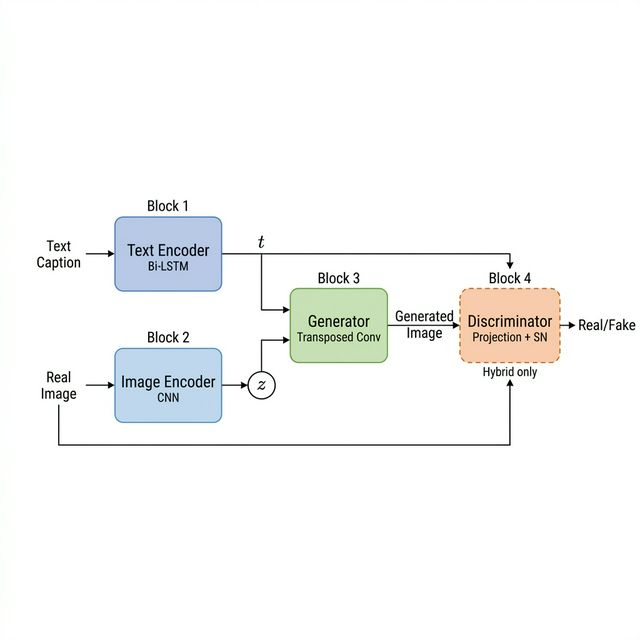
\includegraphics[width=0.95\textwidth]{cvae_gan_architecture.png}
\caption{Architecture of the Hybrid CVAE-GAN model. The discriminator (dashed) is active only in the hybrid variant.}
\label{fig:architecture}
\end{figure}

\subsection{Loss Functions}

The CVAE term is
\[
\mathcal{L}_{\text{CVAE}} = \lambda_{\text{rec}}\,\|x-\hat{x}\|_1 + \lambda_{\text{KL}}\,D_{KL}(q(z|x,t)\|p(z)).
\]

The discriminator hinge loss is
\[
\mathcal{L}_D = \mathbb{E}[\max(0,1-D(x,t))] + \mathbb{E}[\max(0,1+D(\hat{x},t))].
\]

For the hybrid variant, generator training uses
\[
\mathcal{L}_G = \mathcal{L}_{\text{CVAE}} + \lambda_{\text{GAN}}\,\mathcal{L}_{G,\text{hinge}},
\quad
\mathcal{L}_{G,\text{hinge}} = -\mathbb{E}[D(\hat{x},t)].
\]

\section{Experimental Setup}

The comparison protocol is controlled as follows:
\begin{itemize}
\item Variants: \texttt{baseline\_cvae} (GAN disabled) vs \texttt{hybrid\_cvae\_gan} (GAN enabled)
\item Seed: 42
\item Epochs: 10
\item Image size: $64 \times 64$
\item Batch size: 32
\item Optimizer: Adam ($lr_G = lr_D = 2\times 10^{-4}$, $\beta_1=0.5$, $\beta_2=0.999$)
\item Important weights: $\lambda_{\text{KL}}=10^{-3}$, $\lambda_{\text{GAN}}=0.5$
\item Checkpointing: per-epoch checkpoints + best checkpoint by FID
\end{itemize}

Saved artifacts include:
\begin{itemize}
\item Per-run training logs in \texttt{history.csv}
\item Aggregate summary in \texttt{experiment\_summary\_full.csv}
\item Qualitative sample grids in \texttt{runs\_hybrid\_cvae\_gan/sample\_grids}
\end{itemize}

\section{Results}

\subsection{Final Quantitative Comparison}

Table~\ref{tab:main_results} reports final metrics from \texttt{experiment\_summary\_full.csv}.

\begin{table}[H]
\centering
\begin{tabular}{lcccc}
\toprule
Model & FID $\downarrow$ & IS $\uparrow$ & Val Recon $\downarrow$ & Val KL \\
\midrule
Baseline CVAE & 180.66 & 1.41 $\pm$ 0.02 & 0.157 & 37.31 \\
Hybrid CVAE+GAN & 113.52 & 1.83 $\pm$ 0.05 & 0.264 & 39.45 \\
\bottomrule
\end{tabular}
\caption{Final metrics from \texttt{experiment\_summary\_full.csv}.}
\label{tab:main_results}
\end{table}

The hybrid model improves perceptual metrics (FID/IS), while the baseline retains lower reconstruction error.

\subsection{Training Dynamics}

Figure~\ref{fig:training_curves} summarizes metric trajectories across epochs.

\begin{figure}[H]
\centering
\includegraphics[width=0.98\textwidth]{runs_hybrid_cvae_gan/sample_grids/training_curves_metrics.png}
\caption{Per-epoch FID, IS, and validation reconstruction trends for baseline and hybrid variants.}
\label{fig:training_curves}
\end{figure}

The curves indicate earlier and stronger FID gains for the hybrid model, sustained IS advantages, and consistently higher reconstruction loss relative to baseline.

\subsection{Qualitative Comparison and Diversity}

Figure~\ref{fig:fixed_seed} provides fixed-seed side-by-side generations for identical prompts. Figure~\ref{fig:diversity} shows multi-seed diversity for one prompt.

\begin{figure}[H]
\centering
\includegraphics[height=0.72\textheight,keepaspectratio]{runs_hybrid_cvae_gan/sample_grids/fixed_seed_comparison.png}
\caption{Fixed-seed comparison between baseline CVAE and hybrid CVAE+GAN.}
\label{fig:fixed_seed}
\end{figure}

\begin{figure}[H]
\centering
\includegraphics[width=0.95\textwidth]{runs_hybrid_cvae_gan/sample_grids/diversity_grid_dog.png}
\caption{Diversity grid for prompt ``A photo of a dog.'' across multiple seeds.}
\label{fig:diversity}
\end{figure}

\FloatBarrier

Qualitatively, the hybrid variant produces sharper local structure and higher contrast, while the baseline exhibits smoother and blurrier outputs.

\section{Discussion}

The study confirms the intended behavior of the hybrid design: adversarial supervision improves perceptual quality indicators but shifts optimization away from low pixel-level reconstruction error.

The improvement is meaningful for the tested setup, but interpretation should remain bounded by dataset and protocol constraints.

\section{Limitations and Future Work}

Current limitations and immediate extensions include:
\begin{itemize}
\item Captions are class templates rather than rich natural-language descriptions.
\item CIFAR-10 resolution limits semantic and structural fidelity.
\item Results are based on one full seed; multi-seed confidence intervals are needed.
\item Additional alignment metrics (for example CLIP-based scoring) should be incorporated.
\item Evaluation on caption-rich datasets (for example CUB or MS-COCO) is a priority.
\end{itemize}

\section{Ethical Considerations}

Text-to-image systems raise familiar concerns:
\begin{itemize}
\item Misuse for misleading synthetic content
\item Bias inherited from training data
\item Intellectual property and ownership ambiguity
\end{itemize}

Responsible use requires transparent reporting, dataset awareness, and clearly labeling generated content.

\section{Conclusion}

Under matched training conditions, the hybrid CVAE-GAN variant outperforms the CVAE baseline on FID and IS while increasing reconstruction error. Quantitative curves and qualitative grids consistently support the same trade-off: stronger perceptual realism at the cost of pixel-level fidelity. The findings motivate broader evaluation on richer text-image datasets and multi-seed protocols.

\begin{thebibliography}{9}

\bibitem{goodfellow2014}
I. Goodfellow et al., ``Generative Adversarial Nets,'' \textit{NeurIPS}, 2014.

\bibitem{kingma2013}
D. P. Kingma and M. Welling, ``Auto-Encoding Variational Bayes,'' \textit{ICLR}, 2014.

\bibitem{sohn2015}
K. Sohn, H. Lee, and X. Yan, ``Learning Structured Output Representation using Deep Conditional Generative Models,'' \textit{NeurIPS}, 2015.

\bibitem{miyato2018}
T. Miyato and M. Koyama, ``cGANs with Projection Discriminator,'' \textit{ICLR}, 2018.

\bibitem{heusel2017}
M. Heusel et al., ``GANs Trained by a Two Time-Scale Update Rule Converge to a Local Nash Equilibrium,'' \textit{NeurIPS}, 2017.

\bibitem{salimans2016}
T. Salimans et al., ``Improved Techniques for Training GANs,'' \textit{NeurIPS}, 2016.

\bibitem{krizhevsky2009}
A. Krizhevsky, ``Learning Multiple Layers of Features from Tiny Images,'' 2009.

\end{thebibliography}

\end{document}